\documentclass[10pt,a4paper]{article}

\usepackage{commons/course}

\usepackage{listings}
\usepackage{xcolor}

% Define colors for syntax highlighting
\definecolor{keywordstyle}{rgb}{0.0, 0.4, 0.8} % A bluer shade
\definecolor{stringstyle}{rgb}{0.9, 0.17, 0.31} % amaranth
\definecolor{commentstyle}{rgb}{0.1, 0.6, 0.2} % green
\definecolor{numberstyle}{rgb}{0.4, 0.4, 0.4} % gray
\definecolor{backgroundcolor}{rgb}{0.94, 0.97, 1.0} % aliceblue

% Define the Python-like language for syntax highlighting
\lstdefinelanguage{PythonLike}{
	morekeywords={db,capped,size,max,collection,mongoexport,mongoimport,file,out},
	sensitive=false,
	morecomment=[l]{;},
	morestring=[b]",
}




% Set the style for Python-like code
\lstset{
	language=PythonLike,
	basicstyle=\ttfamily\small,
	keywordstyle=\color{keywordstyle},
	stringstyle=\color{stringstyle},
	commentstyle=\color{commentstyle},
	numbers=left,
	numberstyle=\tiny\color{numberstyle},
	stepnumber=1,
	numbersep=5pt,
	keepspaces=true,
	tabsize=4,
	showspaces=false,
	showstringspaces=false,
	showtabs=false,
	breaklines=true,
	breakatwhitespace=false,
	frame=single,
	backgroundcolor=\color{backgroundcolor},
}

\begin{document}

\سربرگ{تمرین پنجم}{}{پاسخ‌دهنده: معین آعلی - 401105561}{استاد: مهدی آخی}



\مسئله{‌}

\section{طرح کوئری }
DBMS
یک کد SQL را به یک طرح کوئری تبدیل می‌کند. عملگرهای طرح کوئری به صورت یک درخت چیده می‌شوند. داده‌ها از برگ‌های این درخت به سمت ریشه این درخت جرکت می‌کنند. خروجی ریشه در درخت نتیجه کوئری است. معمولاً عملگرها باینری (1-2 فرزند دارند) هستند. یک درخت پرس و جو می‌تواند به چندین روش تشکیل و اجرا شود.

\section{مدل‌های پردازشی}
مدل پردازش DBMS مشخص می‌کند که سیستم چگونه یک برنامه پرس و جو را اجرا کند. این مدل چیزهایی مانند جهت ارزیابی کوئری و نوع داده‌هایی که بین عملگرها در طول مسیر منتقل می‌شود را تعیین می‌کند. مدل‌های پردازش مختلفی وجود دارند که برای بارهای کاری مختلف دارای مزایا و معایب متفاوتی نسبت به هم هستند.

این مدل‌ها همچنین می‌توانند به گونه‌ای پیاده‌سازی شوند که عملگرها را از بالا به پایین یا از پایین به بالا فراخوانی کنند. اگرچه رویکرد بالا به پایین بسیار رایج‌تر است، اما رویکرد پایین به بالا می‌تواند کنترل بهتری بر حافظه‌های نهان (کش‌) و ثبات‌ها در خطوط لوله پردازنده فراهم کند.

سه مدل اجرایی که در ادامه مورد بررسی قرار می‌گیرند عبارتند از:


\begin{itemize}
	\item مدل Iterator
	\item مدل Materialization
	\item مدل Vectorized-Batch
\end{itemize}

\subsection{مدل Iterator}

این مدل که به عنوان مدل Pipeline شناخته می‌شود، رایج‌ترین مدل پردازش است و تقریباً توسط هر DBMS مبتنی بر ردیف استفاده می‌شود.

مدل Iterator با پیاده‌سازی یک تابع Next برای هر عملگر در پایگاه داده کار می‌کند. هر Node در برنامه پرس‌وجو تا زمانی که به برگ می‌رسد، Next را بر روی فرزندان خود فراخوانی می‌کند که شروع به ارسال ردیف‌ها به گره‌های پدر خود برای پردازش می‌کنند. 
سپس هر ردیف تا حد امکان به سمت بالا در برنامه پردازش می‌شود قبل از اینکه ردیف بعدی بازیابی شود. این در سیستم‌های مبتنی بر دیسک مفید است زیرا به ما اجازه می‌دهد هر ردیف را در حافظه به طور کامل استفاده کنیم قبل از این که به ردیف یا صفحه بعدی دسترسی پیدا کند. 

\pagebreak

عملگرهای برنامه پرس‌وجو در یک مدل Iterator بسیار قابل ترکیب و آسان برای استدلال هستند زیرا هر عملگر می‌تواند به طور مستقل از عملگرهای پدر یا پسر خود در درخت برنامه پرس‌وجو پیاده‌سازی شود، به شرطی که یک تابع Next را به صورت زیر پیاده‌سازی کند:

\begin{enumerate}
	\item 
	در هر فراخوانی Next ، عملگر یا یک ردیف را برگرداند یا یک پوینتر null .
	\item 
	عملگر باید یک حلقه را پیاده‌سازی کند که Next را بر روی فرزندان خود Call می‌کند تا ردیف‌های آنها را بازیابی کند و سپس آنها را پردازش کند.
	
	به این ترتیب، فراخوانی Next بر روی یک والد، Next را بر روی فرزندان خود فراخوانی می‌کند و در پاسخ گره فرزند ردیف بعدی را که والد باید پردازش کند، برمی‌گرداند.
	
\end{enumerate}


مدل Iterator اجازه می‌دهد تا جایی که ممکن است، DBMS یک ردیف را از طریق عملگرهای مختلف پردازش کند قبل از اینکه ردیف بعدی را بازیابی کند. 

سری کارهایی که برای یک ردیف در برنامه پرس‌وجو انجام می‌شود، یک خط لوله نامیده می‌شود.


برخی عملگرها تا زمانی که فرزندان تمام ردیف‌های خود را ارسال کنند، مسدود می‌شوند. نمونه‌هایی از این عملگرها شامل joins ، زیردرخواست‌ها و مرتب‌سازی‌ها هستند. این عملگرها به عنوان شکننده‌های خط لوله شناخته می‌شوند.

دستور LIMIT به راحتی با این روش کار می‌کند، زیرا یک عملگر می‌تواند فراخوانی Next بر روی فرزندان خود را زمانی که همه ردیف‌های مورد نیاز خود را دارد متوقف کند.


\qquad\qquad\qquad	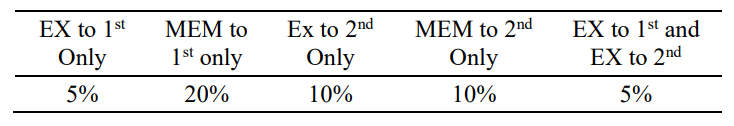
\includegraphics[width=0.7\linewidth]{screenshot001}

در اینجا شبه‌کد برای توابع Next برای هر یک از عملگرها آورده شده است. این توابع Next به طور اساسی حلقه‌های for هستند که بر روی خروجی عملگر فرزند خود تکرار می‌شوند. به عنوان مثال،ریشه Next را بر روی فرزند خود، عملگر join فراخوانی می‌کند. پس از پردازش همه ردیف‌ها، یک پوینتر null (یا پوینتر دیگری) ارسال می‌شود که به گره‌های والد اطلاع می‌دهد که به مرحله بعد بروند.




\pagebreak
\subsection{مدل Materialization‌}

مدل ماده‌سازی یک تخصصی از مدل تکرارگر است که در آن هر عملگر ورودی خود را به طور کامل پردازش کرده و سپس خروجی خود را به طور کامل منتشر می‌کند. به جای داشتن یک تابع Next که یک تاپل را برمی‌گرداند، هر عملگر همه تاپل‌های خود را هر بار که فراخوانی می‌شود، برمی‌گرداند. برای جلوگیری از اسکن تاپل‌های بیش از حد، DBMS می‌تواند اطلاعاتی درباره تعداد تاپل‌های مورد نیاز به عملگرهای بعدی منتقل کند. خروجی می‌تواند یا یک تاپل کامل (NSM) یا یک زیرمجموعه‌ای از ستون‌ها (DSM) باشد.

هر عملگر برنامه پرس‌وجو یک تابع Output را پیاده‌سازی می‌کند که:
\begin{enumerate}
	\item عملگر تمامی ردیف‌ها از فرزندان خود را یکجا پردازش می‌کند.
	
	\item نتیجه بازگشتی از این تابع تمامی ردیف‌هایی است که عملگر هرگز ارسال خواهد کرد. زمانی که عملگر اجرای خود را به پایان می‌رساند، DBMS هرگز نیازی ندارد که برای بازیابی داده‌های بیشتر به آن بازگردد.
\end{enumerate}

این رویکرد برای بارهای کاری OLTP بهتر است زیرا پرس‌وجوها معمولاً تنها به تعداد کمی از ردیف‌ها در هر زمان دسترسی دارند. بنابراین، فراخوانی‌های کمتری برای بازیابی ردیف‌ها وجود دارد. مدل Materialization برای پرس‌وجوهای OLAP با نتایج میانی بزرگ مناسب نیست زیرا ممکن است DBMS نیاز داشته باشد که آن نتایج را بین عملگرها به دیسک منتقل کند.

\qquad\qquad\qquad	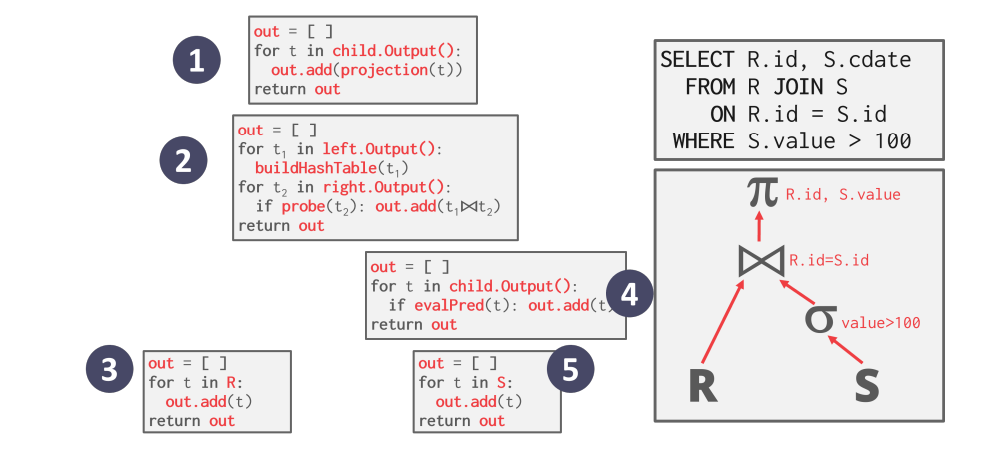
\includegraphics[width=0.7\linewidth]{screenshot002}

در مدل Materialization ، اجرای پرس‌وجو از گره ریشه شروع می‌شود و تابع Output فرزند فراخوانی می‌شود که عملگرهای زیرین را فراخوانی می‌کند و تمامی ردیف‌ها را به سمت بالا باز می‌گرداند. در شکل فوق شبه‌کد برای چگونگی اجرای این فرآیند برای هر عملگر آمده است.

\pagebreak

\subsection{مدل Vectorization}
مانند مدل iterator ، هر عملگر در مدل برداری یک تابع Next را پیاده‌سازی می‌کند. با این حال، هر عملگر یک دسته بردار از داده‌ها را به جای یک تاپل منتشر می‌کند. پیاده‌سازی حلقه داخلی عملگر برای پردازش دسته‌های داده به جای یک مورد در هر زمان بهینه شده است. اندازه دسته می‌تواند بر اساس سخت‌افزار یا ویژگی‌های کوئری متفاوت باشد.

\qquad\qquad\qquad	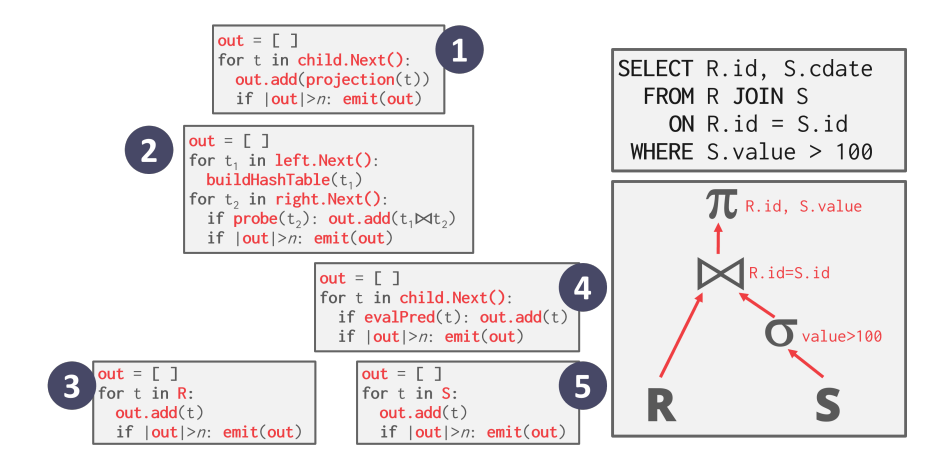
\includegraphics[width=0.7\linewidth]{screenshot003}

مدل بردارسازی بسیار شبیه به مدل Iterator است، به جز اینکه در هر عملگر، یک بافر خروجی با اندازه انتشار مورد نظر مقایسه می‌شود. اگر بافر بزرگتر باشد، یک دسته از ردیف‌ها به بالا ارسال می‌شود. این مدل با پردازش دسته‌ای از ردیف‌ها به جای پردازش تک‌تک ردیف‌ها در هر زمان، بهره‌وری بیشتری را به دست می‌آورد.

مدل بردارسازی به دلیل اینکه تعداد فراخوانی‌های تابع Next کمتر است، برای پرس‌وجوهای OLAP که نیاز به اسکن تعداد زیادی از ردیف‌ها دارند ایده‌آل است. این مدل به عملگرها اجازه می‌دهد تا به راحتی از دستورالعمل‌های برداری (SIMD) برای پردازش دسته‌ای از ردیف‌ها استفاده کنند.

\subsection{جهت پردازش}
\begin{itemize}
	\item رویکرد 1: از بالا به پایین
	\begin{itemize}
		\item با ریشه شروع کنید و داده‌ها را از فرزندان به والدین ``کشیده'' کنید.
		\item تاپل‌ها همیشه با فراخوانی توابع منتقل می‌شوند.
	\end{itemize}
	\item رویکرد 2: از پایین به بالا
	\begin{itemize}
		\item با برگ شروع کنید و داده‌ها را از فرزندان به والدین ``هل'' دهید.
		\item این رویکرد امکان کنترل دقیق‌تر حافظه‌های کش و رجیسترها در خطوط لوله عملگرها را فراهم می‌کند.
	\end{itemize}
\end{itemize}

\pagebreak

\section{روش‌های دسترسی}
به این که DBMS چگونه داده‌های ذخیره شده در یک جدول دسترسی پیدا می‌کند، روش دسترسی میگویند.

به طور کلی دو روش برای مدل‌های دسترسی وجود دارد: داده‌ها یا از یک جدول خوانده می‌شوند یا با یک اسکن ترتیبی از یک شاخص.
\subsection{اسکن ترتیبی}
عملگر اسکن ترتیبی روی هر صفحه در جدول تکرار می‌کند و آن را از حافظه پنهان بافر بازیابی می‌کند. هنگامی که اسکن روی تمام تاپل‌های هر صفحه تکرار می‌کند، گزاره را ارزیابی می‌کند تا تصمیم بگیرد که آیا تاپل را به عملگر بعدی منتشر کند یا نه.


اسکن ترتیبی جدول تقریباً همیشه ناکارآمدترین روش برای اجرای یک پرس و جو توسط یک DBMS است.


تعدادی بهینه‌سازی وجود دارد که به افزایش سرعت اسکن‌های ترتیبی کمک می‌کنند:
\begin{itemize}
	\item پیش‌دریافت: صفحات بعدی را از قبل دریافت کنید تا DBMS مجبور نباشد هنگام دسترسی به هر صفحه بر روی I/O ذخیره‌سازی متوقف شود.
	
	\item دور زدن حافظه پنهان بافر: عملگر اسکن صفحات دریافتی از دیسک را در حافظه محلی خود ذخیره می‌کند تا از سیل ترتیبی جلوگیری کند.
	
	\item موازی‌سازی: اسکن را با استفاده از چندین نخ / فرآیند به صورت موازی اجرا کنید.
	
	\item ماده‌سازی دیرهنگام:
	DBSM های 
	از نوع DSM
	می‌توانند به تأخیر انداختن به هم دوختن توپل‌ها تا بخش‌های بالای طرح پرس و جو را انجام دهند. این اجازه می‌دهد تا هر عملگر حداقل اطلاعات مورد نیاز را به عملگر بعدی منتقل کند.
	
	\item خوشه‌بندی پشته: توپل‌ها با استفاده از یک شاخص خوشه‌بندی در صفحات پشته ذخیره می‌شوند.
	
	\item پرس و جوهای تقریبی: پرس و جوها را بر روی یک زیرمجموعه نمونه‌برداری شده از کل جدول اجرا کنید تا نتایج تقریبی تولید کنید. این به طور معمول برای محاسبه تجمیع‌ها در یک سناریو انجام می‌شود که اجازه خطای کم را می‌دهد تا یک پاسخ تقریباً دقیق تولید شود.
	
	\item نقشه‌بندی منطقه‌ای: پیش‌محاسبه تجمیع‌ها برای هر ویژگی توپل در یک صفحه. DBMS سپس می‌تواند با بررسی نقشه منطقه‌ای خود ابتدا تصمیم بگیرد که آیا نیاز به دسترسی به یک صفحه دارد یا نه.
\end{itemize}

\qquad\qquad\qquad	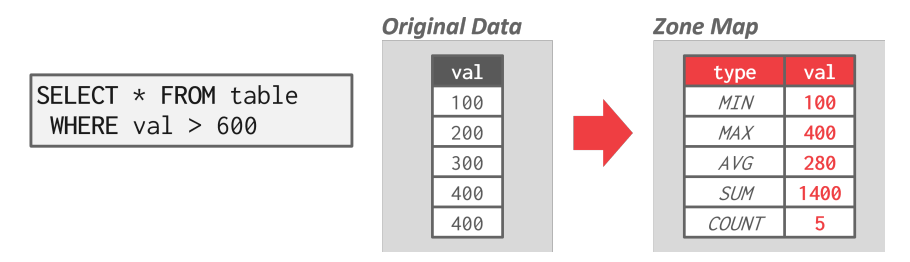
\includegraphics[width=0.7\linewidth]{screenshot004}

در مثال بالا، کوئری Select از Zone-Map متوجه می‌شود که حداکثر مقدار در داده‌های اصلی تنها ۴۰۰ است. 
سپس، به جای آن که مجبور باشد هر زوج مرتب در صفحه را بررسی کند، پرس و جو می‌تواند از دسترسی به صفحه به‌طور کامل اجتناب کند زیرا هیچ یک از مقادیر بزرگتر از ۶۰۰ نخواهند بود.



\subsection{اسکن شاخص}
در یک اسکن شاخص، DBMS یک شاخص را انتخاب می‌کند تا توپل‌هایی که یک پرس و جو نیاز دارد را پیدا کند.

\qquad\qquad\qquad	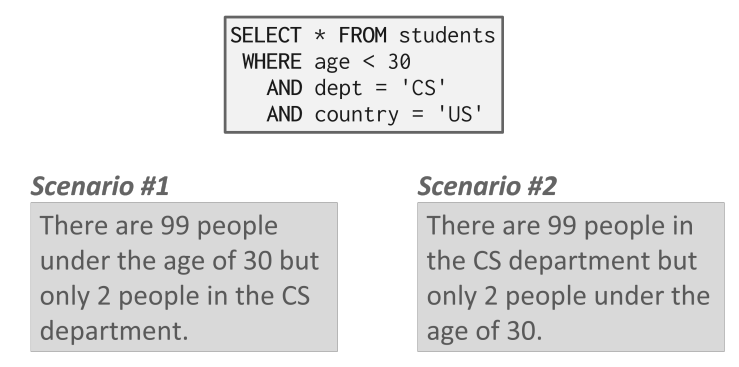
\includegraphics[width=0.7\linewidth]{screenshot005}

جدولی با ۱۰۰ زوج‌مرتب و دو ایندکس را در نظر بگیرید: سن و دپارتمان. 
در سناریوی اول، بهتر است از ایندکس دپارتمان در اسکن استفاده شود زیرا فقط دو زوج‌مرتب برای مطابقت دارد. 
انتخاب ایندکس سن خیلی بهتر از یک اسکن ترتیبی ساده نخواهد بود. 
در سناریوی دوم، ایندکس سن اسکن‌های غیرضروری بیشتری را حذف می‌کند و انتخاب بهینه است.


انتخاب شاخص توسط DBMS شامل عوامل بسیاری است:
\begin{itemize}
	\item چه ویژگی‌هایی در شاخص وجود دارند.
	\item چه ویژگی‌هایی پرس و جو را اشاره می‌کند.
	\item دامنه‌های مقداری ویژگی.
	\item ترکیب گزاره.
	\item اینکه آیا شاخص دارای کلیدهای یکتا یا غیر یکتا است.
\end{itemize}
DBMS
های پیشرفته‌تر از اسکن‌های چند شاخصی پشتیبانی می‌کنند. هنگام استفاده از چندین شاخص برای یک پرس و جو، DBMS مجموعه‌های آیدی های رکوردها را با استفاده از هر شاخص مطابقت داده شده محاسبه می‌کند، این مجموعه‌ها را بر اساس گزاره‌های پرس و جو ترکیب می‌کند، و رکوردها را بازیابی کرده و هر گزاره باقی‌مانده را اعمال می‌کند. DBMS می‌تواند از بیت‌مپ‌ها، جداول هش، یا فیلترهای بلوم برای محاسبه آیدی رکوردها از طریق تقاطع مجموعه‌ها استفاده کند.
\pagebreak

\section{کوئری‌های تعدیلی}
عملگرهایی که پایگاه داده را تغییر می‌دهند مسئول بررسی محدودیت‌ها و به‌روزرسانی شاخص‌ها هستند. 

برای UPDATE/DELETE ، عملگرهای فرزند شناسه‌های رکورد را برای تاپل‌های هدف منتقل می‌کنند و باید تاپل‌های قبلاً دیده شده را ردیابی کنند. دو انتخاب برای نحوه مدیریت عملگرهای INSERT وجود دارد:
\begin{itemize}
	\item انتخاب 1: تاپل‌ها را داخل عملگر ماده‌سازی کنید.
	\item انتخاب 2: عملگر هر تاپل انتقال یافته از عملگرهای فرزند را وارد می‌کند.
\end{itemize}


\qquad\qquad\qquad	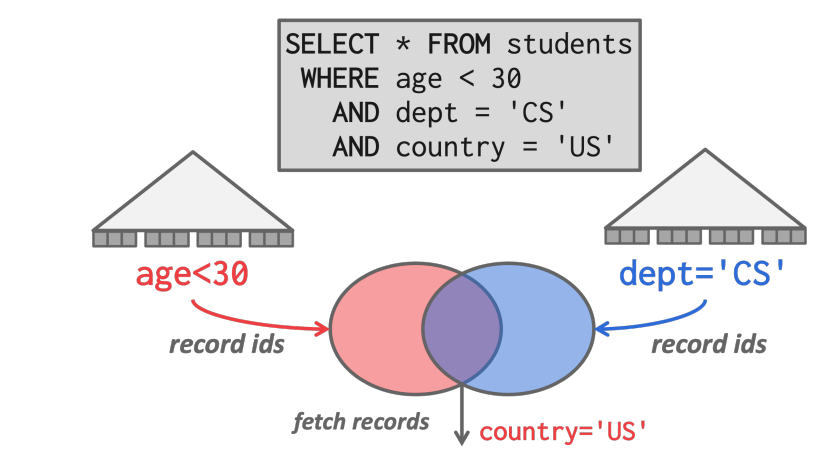
\includegraphics[width=0.7\linewidth]{screenshot006}

همان جدول در شکل قبل را در نظر بگیرید. با پشتیبانی از اسکن چند ایندکسی، ابتدا مجموعه‌های آیدی رکوردها که شرایط برای سن و دپارتمان را برآورده می‌کنند، به ترتیب با استفاده از ایندکس‌های مربوطه محاسبه می‌کنیم. سپس اشتراک دو مجموعه را محاسبه می‌کنیم، رکوردهای مربوطه را واکشی کرده و شرط باقی‌مانده \texttt{country='US'} را اعمال می‌کنیم.



\subsection{مشکل هالووین}
مشکل هالووین یک تناقض است که در آن یک عملیات به‌روزرسانی مکان فیزیکی یک تاپل را تغییر می‌دهد و باعث می‌شود یک عملگر اسکن چندین بار به تاپل مراجعه کند. این می‌تواند در جداول خوشه‌بندی شده یا اسکن‌های شاخص رخ دهد. این پدیده توسط محققان IBM در روز هالووین در سال 1976 هنگام ساخت System R کشف شد. راه حل این مشکل این است که شناسه‌های رکورد اصلاح شده را برای هر کوئری پیگیری شود.

\pagebreak

\section{ارزیابی عبارات}

DBMS
ها یک شرط WHERE را به عنوان یک درخت عبارت نمایش می‌دهد. گره‌ها در این درخت نوع‌های مختلف عبارت را نمایندگی می‌کنند.

\qquad\qquad\qquad	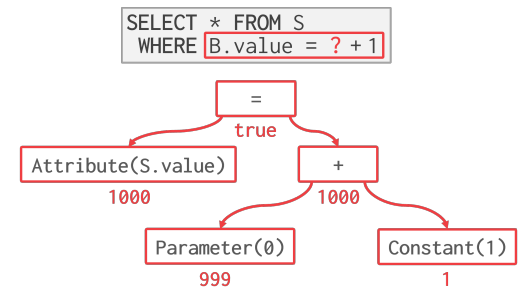
\includegraphics[width=0.7\linewidth]{screenshot007}


برخی از نمونه‌های نوع عبارات که می‌توانند در گره‌های درخت ذخیره شوند:
\begin{itemize}
	\item مقایسه‌ها (=, <, >, !=)
	\item And , Or
	\item عملگرهای حسابی (+, -, *, /, \%)
	\item مقادیر ثابت و پارامتر
	\item مراجع صفت تاپل
\end{itemize}

برای ارزیابی یک درخت عبارت در زمان اجرا، سیستم مدیریت پایگاه داده (DBMS) یک نگهدارنده زمینه را که حاوی فرا داده برای اجرا است، مانند زوج‌مرتب فعلی، پارامترها، و طرحواره جدول، نگهداری می‌کند. سپس DBMS درخت را پیمایش می‌کند تا عملگرهای آن را ارزیابی کرده و نتیجه‌ای تولید کند.

ارزیابی شرایط با این روش کند است زیرا DBMS باید کل درخت را پیمایش کرده و عمل صحیح را برای هر عملگر تعیین کند. رویکرد بهتر این است که عبارت را مستقیماً ارزیابی کنیم. بر اساس مدل هزینه داخلی، DBMS تعیین می‌کند که آیا تولید کد برای تسریع یک پرس‌وجو اتخاذ خواهد شد یا خیر.

\pagebreak
\section{برنامه‌ریز}

مدل‌های پردازش پرس‌وجوی بالا توصیف روشنی از جریان داده ارائه می‌دهند، در حالی که جریان کنترل نسبتاً ضمنی است. زمان‌بند جداسازی روشنی بین جریان داده و جریان کنترل دارد. این روش در حالت دسته‌ای، به‌ویژه مدل بُرداری، به خوبی کار می‌کند. زمان‌بند دستورات کاری را ایجاد می‌کند و به جای فراخوانی درخت عملگر از بالا به پایین، درخت را پیمایش کرده و کارهای زمان‌بندی را در صف زمان‌بندی قرار می‌دهد. سپس رشته‌های کاری درخواست‌ها را از صف واکشی کرده و آنها را اجرا می‌کنند.


\qquad\qquad\qquad	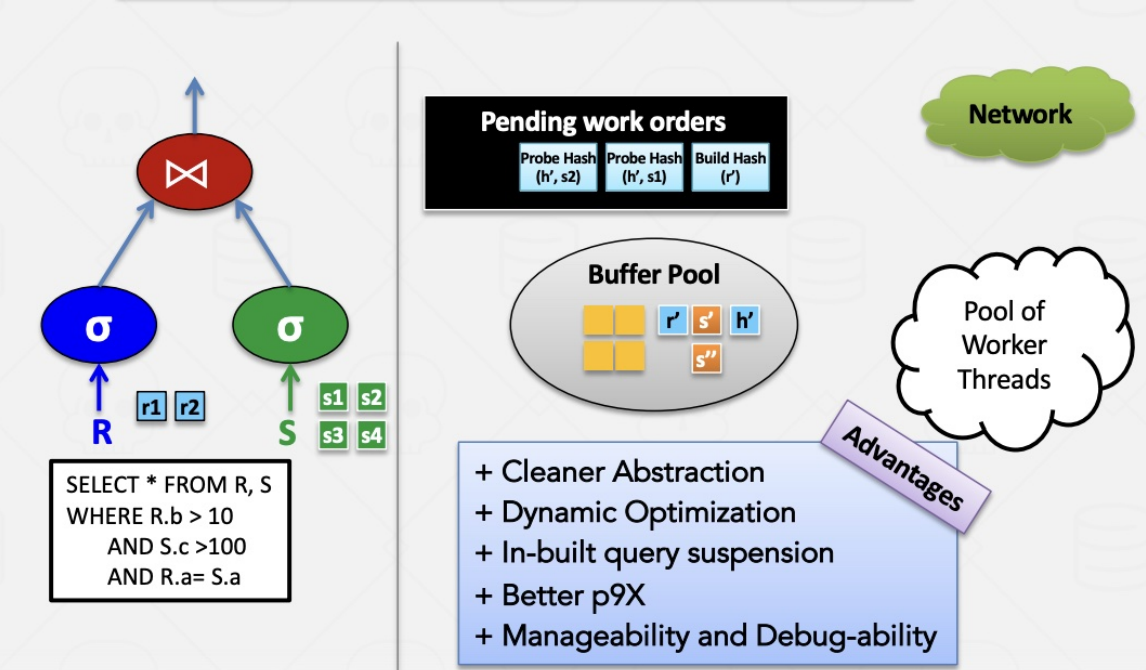
\includegraphics[width=0.7\linewidth]{screenshot008}

در شکل فوق مقایسه مدل پردازش پرس‌وجوی زمان‌بند و مدل پردازش پرس‌وجوی سنتی نشان داده شده است.

به طور کلی، این مدل دارای انتزاع تمیزتر، بهینه‌سازی پویا، تعلیق پرس‌وجوی داخلی، عملکرد بهتر و قابلیت مدیریت و اشکال‌زدایی بهتر است.











\pagebreak


\مسئله{‌}
\section{پیش‌زمینه}
در بحث‌های قبلی اجرای کوئری‌ها فرض بر این بود که کوئری‌ها با یک worker (یعنی thread) اجرا می‌شوند. با این حال، در عمل، کوئری‌ها اغلب به صورت موازی با چندین worker اجرا می‌شوند.
اجرای موازی مزایای کلیدی متعددی برای DBMS ها فراهم می‌کند:
\begin{itemize}
	\item افزایش عملکرد در میزان گذردهی (تعداد بیشتر کوئری‌ها در ثانیه) و زمان پاسخ‌دهی (زمان کمتر برای هر کوئری).
	
	\item افزایش پاسخگویی و دسترس‌پذیری از دید مشتریان خارجی DBMS.
	
	\item کاهش کل هزینه مالکیت. این هزینه شامل هم خرید سخت‌افزار و لایسنس نرم‌افزار، و هم سربار نیروی انسانی برای پیاده‌سازی DBMS و انرژی مورد نیاز برای اجرای ماشین‌ها می‌شود.
\end{itemize}
دو نوع موازی‌سازی وجود دارد که DBMSها پشتیبانی می‌کنند: \lr{inter-query parallelism} و \lr{intra-query parallelism}.

\section{پایگاه‌داده‌های Parallel در مقابل Distributed}
در هر دو سیستم موازی و توزیع‌شده، پایگاه‌داده در میان چندین "منبع" پراکنده شده است تا موازی‌سازی بهبود یابد. این منابع ممکن است محاسباتی (مثل هسته‌های CPU، سوکت‌های CPU، GPUها، ماشین‌های اضافی) یا ذخیره‌سازی (مثل دیسک‌ها، حافظه) باشند.
تمایز بین سیستم‌های موازی و توزیع‌شده مهم است:
\begin{itemize}
	\item \textbf{پایگاه‌داده موازی (Parallel-DBMS)}: در یک پایگاه‌داده موازی، منابع یا گره‌ها از لحاظ فیزیکی به هم نزدیک هستند. این گره‌ها از طریق یک اتصال سریع (high-speed-interconnect) با یکدیگر ارتباط برقرار می‌کنند. فرض بر این است که ارتباط بین منابع نه تنها سریع، بلکه ارزان و قابل اطمینان است.
	
	\item \textbf{پایگاه‌داده توزیع‌شده (Distributed-DBMS)}: در یک پایگاه‌داده توزیع‌شده، منابع ممکن است از هم دور باشند؛ این ممکن است به معنای پراکندگی پایگاه‌داده در قفسه‌ها یا مراکز داده در نقاط مختلف جهان باشد. در نتیجه، منابع از طریق یک اتصال کندتر (اغلب از طریق یک شبکه عمومی) ارتباط برقرار می‌کنند. هزینه‌های ارتباط بین گره‌ها بیشتر است و نمی‌توان از خرابی‌ها چشم‌پوشی کرد.
\end{itemize}
حتی اگر پایگاه‌داده به طور فیزیکی بر روی چندین منبع تقسیم شده باشد، هنوز به صورت یک نمونه پایگاه‌داده منطقی واحد برای برنامه ظاهر می‌شود. بنابراین، یک کوئری SQL که در برابر یک پایگاه‌داده تک‌گره‌ای اجرا می‌شود باید نتیجه یکسانی در یک پایگاه‌داده موازی یا توزیع‌شده تولید کند.


\section{مدل‌های فرآیند}
یک مدل فرآیند DBMS تعیین می‌کند که سیستم چگونه از درخواست‌های همزمان از یک برنامه/محیط چندکاربره پشتیبانی می‌کند. DBMS شامل یک یا چند worker است که مسئول اجرای وظایف به نمایندگی از مشتری و بازگرداندن نتایج هستند. یک برنامه ممکن است یک درخواست بزرگ یا چندین درخواست را به طور همزمان ارسال کند که باید بین workerهای مختلف تقسیم شود.

\qquad\qquad\qquad	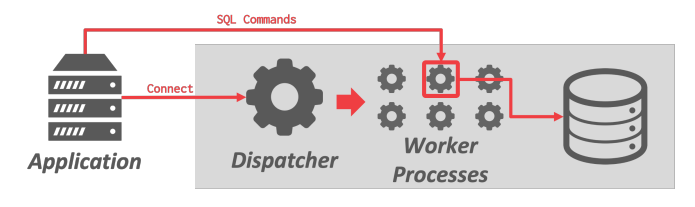
\includegraphics[width=0.7\linewidth]{screenshot009}

دو مدل فرآیند اصلی وجود دارد که یک DBMS ممکن است اتخاذ کند: فرآیند به ازای worker و thread به ازای worker. یک الگوی استفاده رایج دیگر از پایگاه‌داده رویکرد تعبیه شده را اتخاذ می‌کند.

\subsection{Process-per-Worker}
پایه‌ای‌ترین رویکرد، فرآیند به ازای worker است. در اینجا، هر worker یک فرآیند جداگانه سیستم‌عامل است و بنابراین به برنامه‌ریز (scheduler) سیستم‌عامل متکی است. یک برنامه درخواست ارسال می‌کند و یک اتصال به سیستم پایگاه‌داده باز می‌کند. یک توزیع‌کننده (dispatcher) درخواست را دریافت می‌کند و یکی از فرآیندهای worker خود را برای مدیریت اتصال انتخاب می‌کند. برنامه سپس مستقیماً با workerی که مسئول اجرای درخواستی است که کوئری می‌خواهد، ارتباط برقرار می‌کند. این توالی از رویدادها در شکل ۱ نشان داده شده است.

اتکا به سیستم‌عامل برای برنامه‌ریزی به طور موثر کنترل DBMS بر اجرای کارها را کاهش می‌دهد. علاوه بر این، این مدل برای نگهداری ساختارهای داده جهانی به حافظه مشترک متکی است یا به پیام‌رسانی متکی است که سربار بیشتری دارد.

یکی از مزایای رویکرد فرآیند به ازای worker این است که خرابی یک فرآیند کل سیستم را مختل نمی‌کند زیرا هر worker در زمینه فرآیند سیستم‌عامل خود اجرا می‌شود.

این مدل فرآیند مساله کارگران متعدد در فرآیندهای جداگانه که نسخه‌های متعددی از همان صفحه را می‌سازند، ایجاد می‌کند. یک راه‌حل برای به حداکثر رساندن استفاده از حافظه، استفاده از حافظه مشترک برای ساختارهای داده جهانی است تا بتوانند توسط کارگرانی که در فرآیندهای مختلف اجرا می‌شوند، به اشتراک گذاشته شوند.

نمونه‌هایی از سیستم‌هایی که از مدل فرآیند به ازای worker استفاده می‌کنند شامل Postgres و Oracle هستند. زمانی که این DBMSها توسعه یافتند، pthreads هنوز به استاندارد مدل threading تبدیل نشده بود. معنای threading از یک سیستم‌عامل به سیستم‌عامل دیگر متفاوت بود در حالی که \texttt{fork()} بهتر تعریف شده بود.

\subsection{Thread-per-Worker}
مدل رایج امروزی thread به ازای worker است. به جای داشتن فرآیندهای مختلف برای انجام وظایف مختلف، هر سیستم پایگاه‌داده فقط یک فرآیند با چندین thread worker دارد. در این محیط، DBMS کنترل کامل بر وظایف و thread ها دارد و می‌تواند برنامه‌ریزی خود را مدیریت کند. مدل چند thread ممکن است از یک thread توزیع‌کننده استفاده کند یا نکند.

استفاده از معماری چند thread مزایای خاصی فراهم می‌کند. اولاً، سربار کمتری برای هر تعویض زمینه (context switch) وجود دارد. علاوه بر این، نیازی به نگهداری مدل مشترک نیست. با این حال، ممکن است که خرابی یک thread کل فرآیند پایگاه‌داده را از کار بیاندازد. همچنین، مدل thread به ازای worker لزوماً به این معنا نیست که DBMS از موازی‌سازی درون کوئری 
(intra-query-parallelism) پشتیبانی می‌کند.

تقریباً هر DBMS ایجاد شده در ۲۰ سال گذشته از این رویکرد استفاده می‌کند، از جمله SQL Server  و MySQL و Oracle مدل‌های خود را به‌روزرسانی کرده‌اند تا از این رویکرد پشتیبانی کنند. Postgres و پایگاه‌داده‌های مشتق شده از Postgres عمدتاً هنوز از رویکرد مبتنی بر فرآیند استفاده می‌کنند.

\pagebreak

\qquad\qquad\qquad	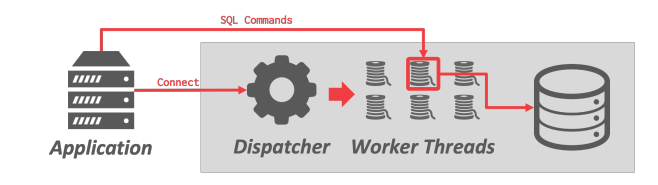
\includegraphics[width=0.7\linewidth]{screenshot011}

\qquad\qquad\qquad	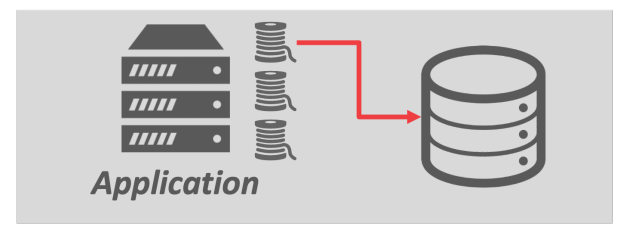
\includegraphics[width=0.7\linewidth]{screenshot012}

\subsection{زمان‌بندی}
در نتیجه، برای هر برنامه کوئری، DBMS باید تصمیم بگیرد کجا، چه زمانی و چگونه اجرا کند. سوالات مرتبط شامل موارد زیر هستند:
\begin{itemize}
	\item از چند وظیفه باید استفاده کند؟
	\item از چند هسته CPU باید استفاده کند؟
	\item وظایف باید روی کدام هسته‌های CPU اجرا شوند؟
	\item خروجی وظیفه باید کجا ذخیره شود؟
\end{itemize}
هنگام تصمیم‌گیری در مورد برنامه‌های کوئری، DBMS همیشه بیشتر از سیستم‌عامل می‌داند و باید به همین ترتیب اولویت داده شود.

\subsection{Embedded-DBMS}
یک الگوی استفاده بسیار متفاوت برای پایگاه‌داده‌ها شامل اجرای سیستم در همان فضای آدرس برنامه است، برخلاف مدل مشتری-سرور که در آن پایگاه‌داده مستقل از برنامه است. در این سناریو، برنامه وظایف و threadها را برای اجرا روی سیستم پایگاه‌داده تنظیم می‌کند. خود برنامه تا حد زیادی مسئول زمان‌بندی خواهد بود. نموداری از رفتارهای زمان‌بندی یک DBMS تعبیه‌شده در شکل ۳ نشان داده شده است.

DuckDB، SQLite و RocksDB مشهورترین DBMSهای تعبیه‌شده هستند.

\pagebreak

\section{موازی‌سازی بین کوئری‌ها (Inter-Query-Parallelism)}
در موازی‌سازی بین کوئری‌ها، DBMS کوئری‌های مختلف را به طور همزمان اجرا می‌کند. از آنجا که چندین worker به صورت همزمان درخواست‌ها را اجرا می‌کنند، عملکرد کلی بهبود می‌یابد. این امر گذردهی را افزایش داده و زمان تاخیر را کاهش می‌دهد.

اگر کوئری‌ها فقط خواندنی باشند، هماهنگی کمی بین کوئری‌ها مورد نیاز است. با این حال، اگر چندین کوئری به طور همزمان در حال به‌روزرسانی پایگاه‌داده باشند، تعارضات پیچیده‌تری ایجاد می‌شود.

\qquad\qquad\qquad	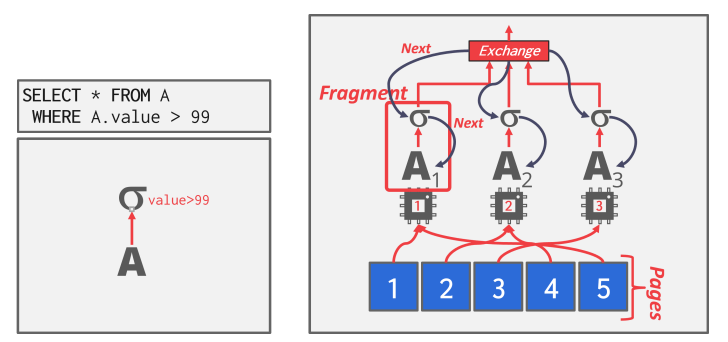
\includegraphics[width=0.7\linewidth]{screenshot013}

برنامه کوئری برای این SELECT یک اسکن ترتیبی روی A است که به یک عملگر فیلتر تغذیه می‌شود. برای اجرای این به صورت موازی، برنامه کوئری به بخش‌های مجزا تقسیم می‌شود. یک بخش برنامه مشخص توسط یک worker متمایز اجرا می‌شود. عملگر تبادل (exchange-operator) به طور همزمان \texttt{Next} را روی همه بخش‌ها فراخوانی می‌کند که سپس داده‌ها را از صفحات مربوطه خود بازیابی می‌کنند.

\section{موازی‌سازی درون کوئری (Intra-Query-Parallelism)}
در موازی‌سازی درون کوئری، DBMS عملیات یک کوئری واحد را به صورت موازی اجرا می‌کند. این امر زمان تاخیر کوئری‌های طولانی‌مدت را کاهش می‌دهد.

سازماندهی موازی‌سازی درون کوئری را می‌توان از دیدگاه پارادایم تولیدکننده/مصرف‌کننده در نظر گرفت. هر عملگر تولیدکننده داده‌ها و همچنین مصرف‌کننده داده‌ها از یک عملگر دیگر که در زیر آن اجرا می‌شود، است. الگوریتم‌های موازی برای هر عملگر رابطه‌ای وجود دارد. DBMS می‌تواند از چندین thread برای دسترسی به ساختارهای داده متمرکز استفاده کند یا از تقسیم‌بندی برای تقسیم کار استفاده کند.

درون موازی‌سازی درون کوئری، سه نوع موازی‌سازی وجود دارد: درون‌عملگر، بین‌عملگر، و بوشی (bushy). این روش‌ها متقابلاً انحصاری نیستند. مسئولیت DBMS این است که این تکنیک‌ها را به گونه‌ای ترکیب کند که عملکرد را بر روی بار کاری داده شده بهینه کند.

\subsubsection{موازی‌سازی درون‌عملگر (افقی)}
در موازی‌سازی درون‌عملگر، عملگرهای برنامه کوئری به بخش‌های مستقل تجزیه می‌شوند که همان عملکرد را بر روی زیرمجموعه‌های متفاوت (مجزا) از داده‌ها انجام می‌دهند.

DBMS یک عملگر تبادل (exchange operator) را در برنامه کوئری درج می‌کند تا نتایج را از عملگرهای فرزند جمع کند. عملگر تبادل از اجرای عملگرهای بالاتر در برنامه تا زمانی که تمام داده‌ها را از فرزندان دریافت کند، جلوگیری می‌کند. نمونه‌ای از این در شکل ۴ نشان داده شده است.
\pagebreak

به طور کلی، سه نوع عملگر تبادل وجود دارد:
\begin{itemize}
	\item \textbf{Gather}: ترکیب نتایج از چندین worker به یک جریان خروجی واحد. این نوع رایج‌ترین نوع مورد استفاده در DBMSهای موازی است.
	\item \textbf{Distribute}: تقسیم یک جریان ورودی به چندین جریان خروجی.
	\item \textbf{Repartition}: سازماندهی مجدد چندین جریان ورودی در چندین جریان خروجی. این امکان را به DBMS می‌دهد که ورودی‌هایی که به یک روش تقسیم شده‌اند را گرفته و سپس به روش دیگری توزیع کند.
\end{itemize}


\subsubsection{موازی‌سازی بین‌عملگر (عمودی)}
در موازی‌سازی بین‌عملگر، DBMS عملگرها را به گونه‌ای همپوشانی می‌کند که داده‌ها را از یک مرحله به مرحله بعدی بدون ماده‌سازی انتقال دهد. این گاهی اوقات به عنوان موازی‌سازی لوله‌ای (pipelined-parallelism) نامیده می‌شود.

\qquad\qquad\qquad	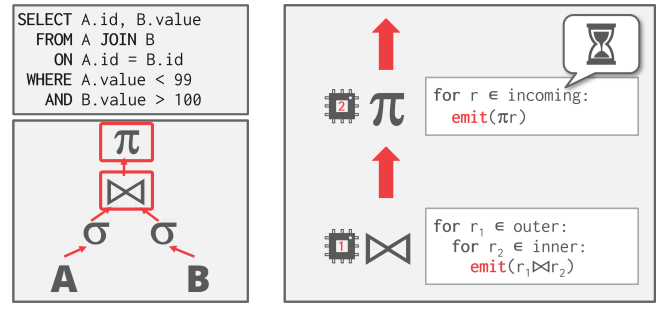
\includegraphics[width=0.7\linewidth]{screenshot014}


در عبارت JOIN سمت چپ، یک worker عملیات join را انجام می‌دهد و سپس نتیجه را به worker دیگری ارسال می‌کند که عملیات projection را انجام می‌دهد و سپس نتیجه را دوباره ارسال می‌کند.

\qquad\qquad\qquad	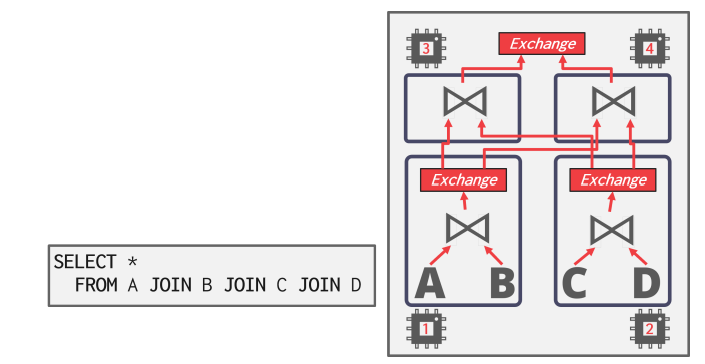
\includegraphics[width=0.7\linewidth]{screenshot015}

برای انجام یک JOIN چهارطرفه روی سه جدول، برنامه کوئری به چهار بخش تقسیم می‌شود همان‌طور که نشان داده شده است. بخش‌های مختلف برنامه کوئری به طور همزمان اجرا می‌شوند، به روشی مشابه با موازی‌سازی بین‌عملگر.
این رویکرد به طور گسترده در سیستم‌های پردازش جریان استفاده می‌شود، که سیستم‌هایی هستند که به طور مداوم یک کوئری را بر روی جریان ورودی tupleها اجرا می‌کنند.

\subsubsection{موازی‌سازی بوشی (Bushy-Parallelism)}
موازی‌سازی بوشی یک ترکیب از موازی‌سازی درون‌عملگر و بین‌عملگر است که در آن worker ها عملگرهای متعدد از بخش‌های مختلف برنامه کوئری را به طور همزمان اجرا می‌کنند.
DBMS همچنان از عملگرهای تبادل برای ترکیب نتایج میانی از این بخش‌ها استفاده می‌کند.


\section{موازی‌سازی I/O}
استفاده از thread اضافی برای اجرای کوئری‌ها به صورت موازی عملکرد را بهبود نمی‌بخشد اگر دیسک همیشه گلوگاه اصلی باشد. بنابراین، مهم است که بتوان پایگاه‌داده را در چندین دستگاه ذخیره‌سازی تقسیم کرد.

برای رفع این مشکل، DBMS ها از موازی‌سازی I/O برای تقسیم نصب بر روی چندین دستگاه استفاده می‌کنند. دو رویکرد برای موازی‌سازی I/O وجود دارد: 
\begin{enumerate}
	\item موازی‌سازی چند دیسک
	\item پارتیشن‌بندی پایگاه‌داده
\end{enumerate}

\subsection{موازی‌سازی چند دیسک}
در موازی‌سازی چند دیسک، سیستم‌عامل/سخت‌افزار برای ذخیره فایل‌های DBMS در چندین دستگاه ذخیره‌سازی پیکربندی می‌شود. این می‌تواند از طریق دستگاه‌های ذخیره‌سازی یا پیکربندی RAID انجام شود. تمام تنظیمات ذخیره‌سازی برای DBMS شفاف است، بنابراین workerها نمی‌توانند بر روی دستگاه‌های مختلف عمل کنند زیرا DBMS از موازی‌سازی زیرساختی آگاه نیست.

\subsection{پارتیشن‌بندی پایگاه‌داده}
در پارتیشن‌بندی پایگاه‌داده، پایگاه‌داده به زیرمجموعه‌های مجزا تقسیم می‌شود که می‌توانند به دیسک‌های مجزا اختصاص داده شوند. برخی از DBMS ها اجازه مشخص کردن مکان دیسک هر پایگاه‌داده فردی را می‌دهند. این کار در سطح سیستم‌فایل آسان است اگر DBMS هر پایگاه‌داده را در یک دایرکتوری جداگانه ذخیره کند. فایل لاگ تغییرات معمولاً به اشتراک گذاشته می‌شود.

ایده پارتیشن‌بندی منطقی این است که یک جدول منطقی واحد به بخش‌های فیزیکی مجزا تقسیم شود که به صورت جداگانه ذخیره/مدیریت می‌شوند. چنین پارتیشن‌بندی به طور ایده‌آل برای برنامه شفاف است. یعنی برنامه باید بتواند به جداول منطقی دسترسی پیدا کند بدون اینکه نگران چگونگی ذخیره‌سازی باشد.

ما این رویکردها را در ادامه ترم و در زمان بحث درباره پایگاه‌داده‌های توزیع‌شده پوشش خواهیم داد.







\pagebreak

\مسئله{‌}
در ابتدا دیتابیس را ساخته و داده‌ها را به آن اضافه می‌کنیم:

\setLTR
\begin{lstlisting}
use airline_tweets;
db.createCollection("tweets");
\end{lstlisting}
\setRTL

\subsection*{الف}
\setLTR
\begin{lstlisting}
db.tweets.find();
\end{lstlisting}
\setRTL
\subsection*{ب}
\setLTR
\begin{lstlisting}
db.tweets.find({"airline_sentiment":"negative"});
\end{lstlisting}
\setRTL
\subsection*{ج}
\setLTR
\begin{lstlisting}
db.tweets.find({
	"airline":"Delta",
	"airline_sentiment": "positive"
});
\end{lstlisting}
\setRTL
\subsection*{د}
\setLTR
\begin{lstlisting}
db.tweets.aggregate([
{
$group: {
	_id: "$airline",
	positive_count: { $sum: { $cond: [{ $eq: ["$airline_sentiment", "positive"] }, 1, 0] } },
	negative_count: { $sum: { $cond: [{ $eq: ["$airline_sentiment", "negative"] }, 1, 0] } },
	neutral_count: { $sum: { $cond: [{ $eq: ["$airline_sentiment", "neutral"] }, 1, 0] } }
	}
}
]);
\end{lstlisting}
\setRTL
\subsection*{ه}
\setLTR
\begin{lstlisting}
db.tweets.find({
	$or: [
	{ "text": { $regex: /Word1/ } },
	{ "text": { $regex: /Word2/ } }
	]
});	
\end{lstlisting}
\setRTL
\subsection*{و}
\setLTR
\begin{lstlisting}
db.tweets.aggregate([
{
	$group: {
		_id: "$airline",
		avg_response_time: { $avg: { $toDate: "$tweet_created" } }
	}
}
]);	
\end{lstlisting}
\setRTL
\pagebreak

\مسئله{‌}
\subsection*{بخش اول}

\subsubsection*{الف}

\setLTR
$\prod_{Name,Type,Quantity}(\sigma_{(eqquipted=True)\land(Registration Date > 2023)}($

 $\qquad \qquad \qquad User \bowtie_{User.userid=Inventory.PlayerID}Inventory$

 $\qquad \qquad \qquad \qquad  \bowtie_{Inventory.InventoryID = InventoryHasItem.InventoryID}InventoryHasItem$
 
 $\qquad \qquad \qquad \qquad  \bowtie_{InventoryHasItem.ItemID=Item.ItemID}Item))$
\setRTL

\subsubsection*{ب}

\setLTR
$ItemWeapons =\prod_{ItemID} (\sigma_{Type=weapon}(Items))$

$FilteredIDs = \prod_{BuyerID}((\prod_{ItemID,BuyerID}Transactions) \text{\textdiv} (ItemWeapons))$

$Usernames =\prod_{username} (FilteredIDs \bowtie_{FilteredIDs.BuyerID = Users.UserID} Users)$
\setRTL

\subsubsection*{ج}

\setLTR
$\prod_{TransactionID}[\sigma_{Transactions.Price>100\$}($

$(Transactions\bowtie_{Transactions.BuyerID=Friends.UserID1 \land Transactions.SellerID=Friends.UserID2}Friends)$

$\bigcup$

$(Transactions\bowtie_{Transactions.SellerID=Friends.UserID1 \land Transactions.BuyerID=Friends.UserID2}Friends))]$

\setRTL
	
\subsection*{بخش دوم}

در این کوئری ابتدا آن بازیکن‌هایی که فروشی نداشته‌اند و XP بزرگتر یا مساوی 250 دارند را آیدی‌شان را جدا کرده، سپس کارکترهای آن‌ها را شناسایی کرده، اگر ویژگی آن کارکترها strength بود اسم آن‌ کارکترها را به ما نشان می‌دهد.

\subsection*{بخش سوم}

کوئری B بهتر است و هزینه اجرای کمتری دارد، زیرا ابتدا روی هر رابطه یک بار Selection کرده و سپس ضرب کارتازین را انجام داده ایم، ولی در کوئری A، ابتدا ضرب را انجام داده و سپس Selection را انجام داده‌ایم، این کار باعث می‌شود که محاسبات اضافی زیادی را انجام بدهیم و Table خود را خیلی خیلی بزرگ کنیم در صورتی که به آن نیازی نداریم. 


\pagebreak

\مسئله{‌}
\subsection*{الف}
\begin{enumerate}
	\item پایگاه‌های داده مستندگرا (Document-oriented):
	این نوع از پایگاه‌های داده برای ذخیره داده‌ها به صورت سند یا مستند استفاده می‌شود. اسناد می‌توانند به صورت JSON نمایش داده شوند و هر سند شامل یک کلید منحصر به فرد برای شناسایی است.
	MongoDB یکی از معروف‌ترین پایگاه‌های داده مستندگرا است که برای برنامه‌هایی که نیاز به ذخیره‌سازی اسناد ساختاری‌نشده و متغیر دارند، مورد استفاده قرار می‌گیرد. برای مثال، برای ذخیره‌سازی اطلاعات کاربران در یک برنامه وب.
	\item پایگاه‌های داده ستونگرا (Column-family):
	در این نوع از پایگاه‌های داده، داده‌ها به صورت ستونی به جای ردیفی ذخیره می‌شوند. این نوع از پایگاه‌های داده به خوبی برای برنامه‌هایی که نیاز به خواندن و نوشتن سریع بر روی داده‌های ستونی دارند، مناسب است. ApacheCassandra  یک نمونه از پایگاه‌های داده ستونگرا است که برای برنامه‌هایی که نیاز به بالا بردن مقیاس پذیری خواندن و نوشتن دارند، مناسب است. برای مثال، در اپلیکیشن‌های شبکه‌های اجتماعی برای ذخیره و بازیابی پست‌ها و اطلاعات کاربران.
	\item پایگاه‌های داده گراف (Graph):
	در این نوع از پایگاه‌های داده، روابط بین داده‌ها به عنوان یال‌ها نمایش داده می‌شوند و اطلاعات به صورت گرافی ذخیره می‌شوند. این نوع پایگاه‌های داده برای مواردی که تحلیل شبکه‌ها یا روابط بین داده‌ها اساسی است، مناسب است.
	$Neo4j$ یک پایگاه داده گراف است که برای ذخیره‌سازی و مدیریت داده‌هایی که ارتباطات بین موجودیت‌ها مهم هستند (مانند شبکه‌های اجتماعی، شبکه‌های موجودیت-ارتباط، موتور جستجوی گرافی و ...) استفاده می‌شود.
	\item پایگاه‌های داده کلید-مقدار (Key-Value):
	در این نوع از پایگاه‌های داده، داده‌ها به صورت جفت‌های کلید و مقدار ذخیره می‌شوند. این نوع پایگاه‌های داده برای کاربردهایی که سادگی در ذخیره و بازیابی داده‌ها و عملیات سریع کلیدی است، بسیار مناسب است.
	Redis یک پایگاه داده کلید-مقدار است که برای ذخیره‌سازی اطلاعات مانند کش، جلسات کاربر، صف‌های پیام و دیگر کاربردهایی که به سرعت بالا در خواندن و نوشتن نیاز دارند، استفاده می‌شود.
	
	
\end{enumerate}
\subsection*{ب}

پایگاه‌های داده NoSQL به خوبی قابلیت افزودن سرورها و توزیع بار را دارند. این به این معنی است که می‌توانند به راحتی با تعداد کاربران، حجم داده یا تراکنش‌های درخواستی افزایش یابند بدون اینکه عملکرد سیستم به شدت تحت فشار قرار بگیرد. مثلاً، در برنامه‌های وبی که تعداد کاربران ممکن است به طور ناگهانی افزایش یابد، مانند پلتفرم‌های شبکه‌های اجتماعی یا خدمات استریمینگ ویدیویی مانند Netflix، پایگاه‌های داده NoSQL می‌توانند با افزودن سرورها به راحتی این مقیاس‌پذیری را فراهم کنند.

در برخی از برنامه‌ها نیاز است که داده‌ها به صورت مستند، ستونی، گراف یا کلید-مقدار ذخیره شوند. پایگاه‌های داده NoSQL به انواع مختلف ساختارهای داده پشتیبانی می‌کنند و این امکان را فراهم می‌کنند که بر اساس نیاز برنامه ساختار داده‌ای را انتخاب کنید.
 بسیاری از پایگاه‌های داده NoSQL برای عملیات خواندن و نوشتن سریع بهینه شده‌اند. به عنوان مثال، پایگاه داده Redis برای کش و مدیریت داده‌های حافظه میانی کارایی بسیار بالایی دارد که برای برنامه‌هایی که نیاز به پاسخگویی فوری دارند، بسیار مناسب است.
 
فرض کنید یک شرکت فروشگاهی آنلاین دارید که در اوج فصل خرید ممکن است با ترافیک بسیار بالا و نوسانات قابل توجه در تعداد کاربران مواجه شود. برای ذخیره و بازیابی سریع اطلاعات سفارشات، مشتریان، و محصولات، می‌توانید از پایگاه داده NoSQL مانند MongoDB استفاده کنید. MongoDB به دلیل قابلیت مقیاس‌پذیری افزایشی خوبش، که به راحتی می‌توانید با افزودن سرورها به تعداد نیاز، ترافیک را مدیریت کنید و به داده‌های پیچیده و پویا نیز پاسخ دهید.

\subsection*{ج}
پایگاه‌های داده NoSQL در تجزیه و تحلیل داده‌های پیچیده و مدیریت تراکنش‌ها ممکن است با محدودیت‌هایی مواجه شوند:
\begin{enumerate}


	\item پشتیبانی متناسب با تراکنش‌های پیچیده: برخی از پایگاه‌های داده NoSQL معمولاً برای مدیریت تراکنش‌های پیچیده مانند تراکنش‌های متقابل یا تراکنش‌های چند مرحله‌ای، پشتیبانی نمی‌کنند به دلیل معماری خودکارتی و بدون تراکنشی که دارند.

\item کنترل دقیق تراکنش‌ها: در پایگاه‌های داده NoSQL، کنترل دقیق تراکنش‌ها به صورتی که در ACID (Atomicity, Consistency, Isolation, Durability) تعریف شده است، معمولاً ضعیفتر است. این ممکن است برای برنامه‌هایی که نیاز به تضمینات دقیق تراکنشی دارند، مشکل ایجاد کند.

\item پرس و جوهای پیچیده: در برخی موارد، پایگاه‌های داده NoSQL ممکن است نتوانند به خوبی پرس و جوهای پیچیده و بازیابی داده‌های پیچیده را پشتیبانی کنند، مخصوصاً اگر نیاز به عملیاتی مانند پیوندهای پیچیده بین داده‌ها داشته باشید.
\end{enumerate}

راه‌حل‌هایی برای این محدودیت‌ها شامل:
\begin{enumerate}

\item  استفاده از پایگاه‌های داده هیبرید: این راه‌حل شامل استفاده از یک ترکیب از پایگاه‌های داده NoSQL برای انعطاف‌پذیری و پایگاه‌های داده رابطه‌ای برای انجام تراکنش‌های پیچیده و حفظ دقت تراکنش‌ها است.

\item  استفاده از مدل‌های معماری پیچیده‌تر: ممکن است نیاز باشد که مدل‌های معماری پیچیده‌تری را در نظر بگیرید تا بتوانید تراکنش‌های پیچیده را به خوبی مدیریت کنید.

\item  استفاده از ابزارهای مدیریت تراکنش: برخی از پایگاه‌های داده NoSQL ابزارهایی برای مدیریت تراکنش‌ها ارائه می‌دهند که می‌تواند به شما کمک کند که تراکنش‌هایی را که نیاز به دقت بالا دارند، مدیریت کنید.

\end{enumerate}








\subsection*{د}
مزایا:
\begin{enumerate}

	\item  مقیاس‌پذیری افزایشی:

پایگاه‌های داده توزیع‌شده در NoSQL به راحتی می‌توانند با افزودن سرورها و منابع جدید، به مقیاس‌پذیری افزایشی پاسخ دهند. این به معنای افزایش ظرفیت ذخیره‌سازی و پردازش است که بدون نیاز به تغییرات زیرساختی بزرگ، انجام می‌شود.
	\item  کارایی بالا:

پایگاه‌های داده توزیع‌شده معمولاً قابلیت عملیات سریع خواندن و نوشتن را دارند، زیرا داده‌ها در سرورهای مختلف قرار می‌گیرند و بار مورد نیاز بین این سرورها توزیع می‌شود.
	\item  استقرار و مقیاس‌پذیری آسان:

نصب و راه‌اندازی پایگاه‌های داده توزیع‌شده معمولاً آسان‌تر از پایگاه‌های داده مرکزی است و می‌توانند به راحتی بر روی سیستم‌های مختلف و با انواع معماری‌ها مستقر شوند.
	\item  انعطاف‌پذیری بالا:

این نوع از پایگاه‌های داده بهترین پاسخ را به محیط‌هایی که نیاز به انعطاف‌پذیری بالا و تغییرات سریع دارند، می‌دهند. می‌توان به سرعت ساختار داده‌ای را تغییر داد و با نیازهای جدید سازگاری بخشید.
\end{enumerate}
\pagebreak
چالش ها:
\begin{enumerate}
\item  هماهنگی داده:
	
	یکی از چالش‌های اصلی پایگاه‌های داده توزیع‌شده، هماهنگی و همگرایی داده‌ها است. تضمین اینکه داده‌ها به درستی و به طور یکسان در تمامی نقاط شبکه توزیع شده باقی مانده باشند، می‌تواند چالشی بزرگ باشد.
\item  مدیریت پویا:
	
	مدیریت پویا و مداوم منابع و توزیع بار به طور اتوماتیک در پایگاه‌های داده توزیع‌شده نیازمند سیستم‌های مدیریت پیچیده‌ای است که این می‌تواند یک چالش مدیریتی باشد.
\item  بهره‌وری در سطح شبکه:
	
	پایگاه‌های داده توزیع‌شده نیازمند بهره‌وری در سطح شبکه بالا هستند. عدم بهره‌وری می‌تواند به تأخیرهای بزرگ و مشکلات در عملکرد سیستم منجر شود.
\item  امنیت:
	
	حفظ امنیت داده‌ها در یک محیط توزیع‌شده نیز یک چالش مهم است. این شامل مسائلی مانند کنترل دسترسی، رمزنگاری و حفاظت در مقابل حملات مختلف می‌شود.
\end{enumerate}
\subsection*{ه}
این قضیه می‌گوید که یک سیستم پایگاه‌داده توزیع‌شده نمی‌تواند همزمان سه ویژگی Consistency (سازگاری), Availability (دسترسی‌پذیری), و PartitionTolerance (مقاومت در برابر جداشدگی) را به صورت کامل داشته باشد.

پایگاه‌های داده NoSQL تلاش می‌کنند تا این سه ویژگی را در محیط‌های توزیع‌شده بهینه‌سازی کنند و بهترین ترکیب بین آنها را ارائه دهند:

\begin{enumerate}
	\item Consistency
	
	برخی از پایگاه‌های داده NoSQL، به جای سازگاری محکم (Strong Consistency)، از یک سازگاری ضعیف‌تر (Weak Consistency) استفاده می‌کنند. این به معنای این است که تاخیرهایی در همگرایی داده‌ها بین نقاط شبکه ممکن است و در نتیجه ممکن است برخی از کلاینت‌ها دیدگاهی متفاوت از داده داشته باشند.
	\item 
	Availability
	
	پایگاه‌های داده NoSQL معمولاً بر روی دسترسی پذیری بالا تمرکز دارند. با افزودن سرورها و توزیع بار، سعی می‌کنند تا همیشه به درخواست‌های کلاینت‌ها پاسخ دهند حتی در صورت اتفاقات ناخواسته مانند قطعی در بخشی از شبکه.
	\item 
	PartitionTolerance
	
	تقریباً همهٔ پایگاه‌های داده NoSQL بر روی مقاومت در برابر جداشدگی تمرکز دارند. آنها طراحی شده‌اند تا بتوانند با قطعی شبکه یا مشکلات دیگر مانند تاخیر‌ها در انتقال داده، همچنان به طور صحیح عمل کنند.
\end{enumerate}

پایگاه‌های داده NoSQL از طریق استفاده از تکنیک‌های مختلف مانند انتخاب مناسب روش‌های Replication (تکثیر)، Sharding (شاردینگ)، و Consistency Models (مدل‌های سازگاری)، سعی می‌کنند که تعادل مناسبی بین 3 ویژگی فراهم کنند تا بهترین عملکرد را در محیط‌های توزیع‌شده ارائه دهند.
\pagebreak

\subsection*{و}
مزایا:

\begin{enumerate}
	\item جستجوی سریع و بازیابی داده:
	
	شاخص‌گذاری به سرعت و کارایی در جستجوها و بازیابی داده‌ها کمک می‌کند. با استفاده از شاخص‌ها، عملیات جستجو و فیلترینگ داده‌ها به سرعت انجام می‌شود.
	
	\item پاسخگویی بهتر به درخواست‌های پیچیده:
	
	با استفاده از شاخص‌گذاری، می‌توان به سریعی و با کارایی به درخواست‌های پیچیده مانند جستجوهای با چندین شرط پاسخ داد.
	\item مرتب‌سازی و گروه‌بندی بهتر:
	
	شاخص‌گذاری به مرتب‌سازی و گروه‌بندی داده‌ها بر اساس فیلدهای مختلف کمک می‌کند، که این موضوع برای تجزیه و تحلیل داده‌ها و استفاده‌های مختلف بسیار مفید است.
	\item کاهش زمان اجرا و بار مورد نیاز:
	
	با استفاده از شاخص‌گذاری، زمان اجرا و بار مورد نیاز برای اجرای عملیات‌های مختلف را می‌توان به حداقل رساند.
\end{enumerate}

معایب:

\begin{enumerate}
\item هزینه ذخیره‌سازی اضافی:
	
	ایجاد شاخص‌های زیاد ممکن است نیاز به فضای ذخیره‌سازی اضافی داشته باشد، خصوصاً اگر داده‌ها بزرگ باشند.
\item هزینه محاسباتی بالا برای بروزرسانی شاخص‌ها:
	
	بروزرسانی شاخص‌ها ممکن است به هزینه محاسباتی زیادی منجر شود، به خصوص اگر داده‌ها پویا باشند و بروزرسانی مداومی نیاز داشته باشد.
\item پیچیدگی مدیریت شاخص‌ها:
	
	مدیریت و نگهداری شاخص‌ها و اطمینان از اینکه همیشه به‌روز هستند، می‌تواند پیچیده و زمان‌بر باشد.
\end{enumerate}

بهینه سازی:
\begin{enumerate}
\item انتخاب شاخص‌های مناسب:
	
	انتخاب دقیق و منطقی شاخص‌ها بر اساس نیازهای واقعی برنامه و عملکرد پایگاه داده مهم است. شاخص‌هایی که بیشترین تأثیر را بر عملکرد دارند و بیشترین بهره را از حافظه و پردازنده دارند، باید در اولویت قرار گیرند.
	\item بهینه‌سازی فرآیند بروزرسانی:
	
	برای کاهش هزینه محاسباتی بروزرسانی شاخص‌ها، می‌توان از روش‌های بهینه‌سازی مانند استفاده از شاخص‌های گسترده‌تر (WideIndexes) به جای شاخص‌های عمیق (DeepIndexes) استفاده کرد.
	\item مانیتورینگ و بهبود مداوم:
	
	مدیریت مداوم شاخص‌ها، نظارت بر کارایی آنها و به‌روزرسانی آنها با توجه به تغییرات در الگوهای داده‌ها و نیازهای برنامه می‌تواند به بهبود عملکرد کمک کند.
\end{enumerate}

\subsection*{ز}

پایگاه‌های داده NoSQL معمولاً از ساختار داده‌ای انعطاف‌پذیری استفاده می‌کنند. به جای ساختارهای رابطه‌ای (مانند جداول در پایگاه‌های داده رابطه‌ای)، از مدل‌های مختلفی مانند مدل سندی (MongoDB)، مدل ستونی (Cassandra)، یا مدل کلید-مقدار (Redis) استفاده می‌کنند که به طور طبیعی از انعطاف‌پذیری بالایی برخوردار هستند.
این نوع از پایگاه‌های داده به خوبی تغییرات پویا در ساختار داده‌ها را پذیرفته و مدیریت می‌کنند. به دلیل عدم وجود یک سکونت سخت در ساختار داده، می‌توان به راحتی فیلدها یا ویژگی‌های جدید را به مدل داده اضافه کرد یا حتی فیلدهای موجود را حذف یا تغییر داد.
در پایگاه‌های داده NoSQL، معمولاً از شیوه‌های ذخیره و بازیابی انعطاف‌پذیری استفاده می‌شود که امکان مدیریت داده‌های پویا را فراهم می‌کند. به عنوان مثال، در MongoDB، می‌توان به راحتی یک سند جدید با فیلدهای جدید اضافه کرد و این تغییرات به سرعت در سراسر سیستم توزیع‌شده پخش می‌شود.

مزایا:

\begin{enumerate}
	\item 	 پاسخگویی به نیازهای تغییرات سریع در برنامه‌ها:

	این ویژگی به توسعه‌دهندگان اجازه می‌دهد که به راحتی تغییرات در نیازهای برنامه و ساختار داده‌ای را اعمال کنند بدون اینکه نیاز به تغییرات گسترده در ساختار پایگاه داده داشته باشند.
	\item 	 افزایش سرعت توسعه و تحویل محصول:
	
	با اینکه به راحتی می‌توان ساختار داده را تغییر داد، سرعت توسعه و تحویل محصول افزایش می‌یابد. تیم‌های توسعه می‌توانند با سرعت بیشتری واکنش نشان دهند و نسبت به بازخوردهای کاربران و نیازهای بازار واکنش نشان دهند.
	\item 	 انعطاف‌پذیری در تجزیه و تحلیل داده‌ها:
	
	انعطاف‌پذیری در ساختار داده‌ها به تحلیل‌گران و دانشمندان داده امکان می‌دهد که به سرعت به تغییرات در نیازهای تحلیلی و گزارش‌دهی پاسخ دهند و به تحلیل‌های پیچیده‌تر دست پیدا کنند.
\end{enumerate}

\subsection*{س}
مزایا:
\begin{enumerate}
\item  کارایی بالا:
	
	استفاده از قوام نهایی معمولاً منجر به کارایی بالاتری می‌شود، زیرا این مدل اجازه می‌دهد که عملیات خواندن داده‌ها بدون نیاز به انتظار تطابق نهایی (consistency) انجام شود. این به این معنی است که درخواست‌های خواندن به سرعت اطلاعات را از نواحیی که به‌روزرسانی نشده‌اند، دریافت می‌کنند.
\item  مقیاس‌پذیری بهتر:
	
	در سیستم‌های توزیع‌شده، مانند پایگاه‌های داده NoSQL، مقیاس‌پذیری بسیار مهم است. قوام نهایی امکان افزایش مقیاس‌پذیری سیستم را بدون تاثیر زیاد بر عملکرد اجازه می‌دهد، زیرا نیاز به همگام‌سازی فوری بین تمامی نقاط سیستم وجود ندارد.
\item  منعطف‌سازی در تاخیرهای شبکه:
	
	در شبکه‌های بزرگ و پیچیده، تاخیرها ممکن است متفاوت باشند. قوام نهایی به سیستم اجازه می‌دهد تا با تاخیرهای شبکه سازگار باشد و به جای تلاش برای همگام‌سازی فوری، در نهایت به تطابق بپردازد.
\end{enumerate}
\pagebreak
مواردی که مناسب نیست:
\begin{enumerate}
\item  نیاز به کنترل دقیق تر Consistency
	
	در برخی از برنامه‌ها و استفاده‌های که نیاز به انطباق دقیق بین داده‌ها در تمامی نقاط سیستم دارند (مانند تراکنش‌های مالی یا سامانه‌های حساس به اطلاعات)، قوام نهایی ممکن است مناسب نباشد. این امر می‌تواند منجر به ایجاد مشکلاتی مانند دوگانگی داده‌ها یا افزایش خطرات امنیتی شود.
\item  نیاز به تضمین دقیق زمان پاسخگویی
	
	در برخی از سرویس‌ها و برنامه‌ها، نیاز به تضمین دقیق زمان پاسخگویی (Service Level Agreement) وجود دارد. استفاده از قوام نهایی ممکن است این تضمین را دشوار کند زیرا زمانی که لازم است تا داده‌ها به طور کامل همگام شوند، قابل پیش‌بینی نیست.
\item  نیاز به جلوگیری از دوگانگی داده
	
	در برخی موارد، نیاز است که داده‌ها از دوگانگی جلوگیری شود و همگام‌سازی فوری بین تمامی نقاط سیستم ضروری است تا این اتفاق رخ ندهد. قوام نهایی این نیاز را برآورده نمی‌کند و ممکن است داده‌ها در نقاط مختلف سیستم دوباره ذخیره شوند.
\end{enumerate}


\subsection*{ش}
ACID مخفف Atomicity (اتمیتی)، Consistency (سازگاری)، Isolation (عزلت)، Durability (پایداری) است.

\begin{itemize}
	\item عملیات یک تراکنش باید به طور کامل یا همه‌پرسی (یا همه‌گیری) انجام شود یا به طور کامل نتیجه‌ای نداشته باشد. به عبارت دیگر، هیچگاه نباید به وضعیت نیمه‌کامل برسد.	
	
	\item پایگاه داده همیشه باید در یک وضعیت صحیح و معتبر باشد، چه قبل، چه بعد از هر تراکنشی.
	
	\item هر تراکنش باید مستقل از دیگری اجرا شود و تأثیر یک تراکنش نباید بر تراکنش‌های دیگر تأثیر بگذارد.
	
	\item پس از انجام یک تراکنش موفق، تغییرات اعمال شده باید دائمی باشند و در برابر خرابی سیستم مقاوم باشند.
\end{itemize}

پایگاه داده‌های رابطه‌ای مانند MySQL یا PostgreSQL: این پایگاه‌های داده از مدل ACID پیروی می‌کنند و تضمین می‌کنند که تراکنش‌ها به طور کامل، با سازگاری، عزلت، و پایداری اجرا می‌شوند.
$\\ \\$

BASE نام اختصاری است از BasicallyAvailable (در دسترس بودن در اساس)، Soft state (وضعیت نرم)، EventuallyConsistent (سازگاری در نهایت). این مدل بر اصول زیر تمرکز دارد:

\begin{itemize}
	\item سیستم باید به طور مداوم در دسترس باشد، حتی با قیودی بر روی Consistency داده‌ها.
	\item وضعیت داده‌ها ممکن است در طول زمان تغییر کند و در یک زمان داده‌ها ممکن است به طور کامل همگام نباشند.
	\item در نهایت، داده‌ها باید به وضعیتی برسند که سازگاری داشته باشند، حتی اگر بین انتقال و تغییرات داده‌ها تأخیر وجود داشته باشد.	
\end{itemize}

پایگاه داده‌های NoSQL مانند Cassandra یا Riak بر اساس مدل BASE عمل می‌کنند. آنها تلاش می‌کنند که در دسترس باشند (BasicallyAvailable)، وضعیت نرم دارند (SoftState)، و سازگاری در نهایت را تضمین می‌کنند (EventuallyConsistent).

\subsection*{ص}
 پایگاه‌های داده NoSQL با امکانات متنوعی که ارائه می‌دهند، می‌توانند برای ذخیره و تحلیل داده‌های جغرافیایی مناسب باشند، اما قبل از انتخاب و استفاده، باید چالش‌های مرتبط را در نظر گرفته و راه‌حل‌های مناسب برای آنها ارائه داد.

مزایا:
\begin{enumerate}
\item  پشتیبانی از انواع داده‌ساختارها:
	
	پایگاه‌های داده NoSQL از انواع مختلف ساختارهای داده پشتیبانی می‌کنند که از جمله آنها می‌توان به ساختارهای جغرافیایی مانند نقطه، خط، پلیگون، و حتی مجموعه‌های داده جغرافیایی اشاره کرد. این امکان را فراهم می‌کنند که داده‌های مکانی و جغرافیایی را به صورت مستقیم ذخیره و مدیریت کرد.
	\item  مقیاس‌پذیری و عملکرد:
	
	بسیاری از پایگاه‌های داده NoSQL برای مقیاس‌پذیری عالی طراحی شده‌اند، به طوری که می‌توانند حجم بالای داده‌های جغرافیایی را به خوبی مدیریت کنند و همچنین در عملیات خواندن و نوشتن سریع عمل کنند. این ویژگی برای سیستم‌هایی که نیاز به پردازش و تحلیل زنده داده‌های جغرافیایی دارند، بسیار مهم است.
	\item  امکان پرس‌وجوی پیچیده:
	
	پایگاه‌های داده NoSQL معمولاً امکاناتی برای پرس‌وجوهای پیچیده بر روی داده‌های جغرافیایی ارائه می‌دهند، مانند پرس‌وجوهای مکانی (SpatialQueries)، پرس‌وجوهای نزدیکی (ProximityQueries)، و پرس‌وجوهای بازه‌ای (RangeQueries) که برای تحلیل داده‌های جغرافیایی بسیار مفید هستند.
\end{enumerate}


چالش ها:

\begin{enumerate}
	\item پایداری و همگام‌سازی:
	
	در پایگاه‌های داده NoSQL که به صورت توزیع‌شده عمل می‌کنند، مدیریت پایداری داده‌ها و همگام‌سازی آنها می‌تواند چالش بزرگی باشد، به خصوص زمانی که نیاز به تطابق دقیق بین داده‌های جغرافیایی در مناطق مختلف وجود دارد.
	\item پیچیدگی پرس‌وجو:
	
	برخی پایگاه‌های داده NoSQL ممکن است نهایتاً سازگاری را برای داده‌های جغرافیایی ارائه کنند، اما این ممکن است با پیچیدگی‌هایی در پیکربندی و اجرای پرس‌وجوهای پیچیده همراه باشد که نیاز به آموزش و تجربه داشته باشد.
	\item مدیریت حجم بالای داده‌ها:
	
	داده‌های جغرافیایی معمولاً حجم بالایی دارند و برای مدیریت این حجم بزرگ از دیسک و حافظه میانی نیاز است که برخی پایگاه‌های داده NoSQL ممکن است به دشواری با آنها مقابله کنند.
\end{enumerate}
\end{document}